% vim: tw=80:conceallevel=0
\documentclass[times, utf8, diplomski]{fer}
\usepackage{booktabs}
\usepackage{float}
\usepackage{pdfpages}

\begin{document}

\thesisnumber{2902}

\title{Razvoj informacijskog sustava za potporu organizaciji događanja s velikim
brojem sudionika korištenjem programskog okvira za ubrzani razvoj aplikacija}

\author{Fran Borčić}

\maketitle

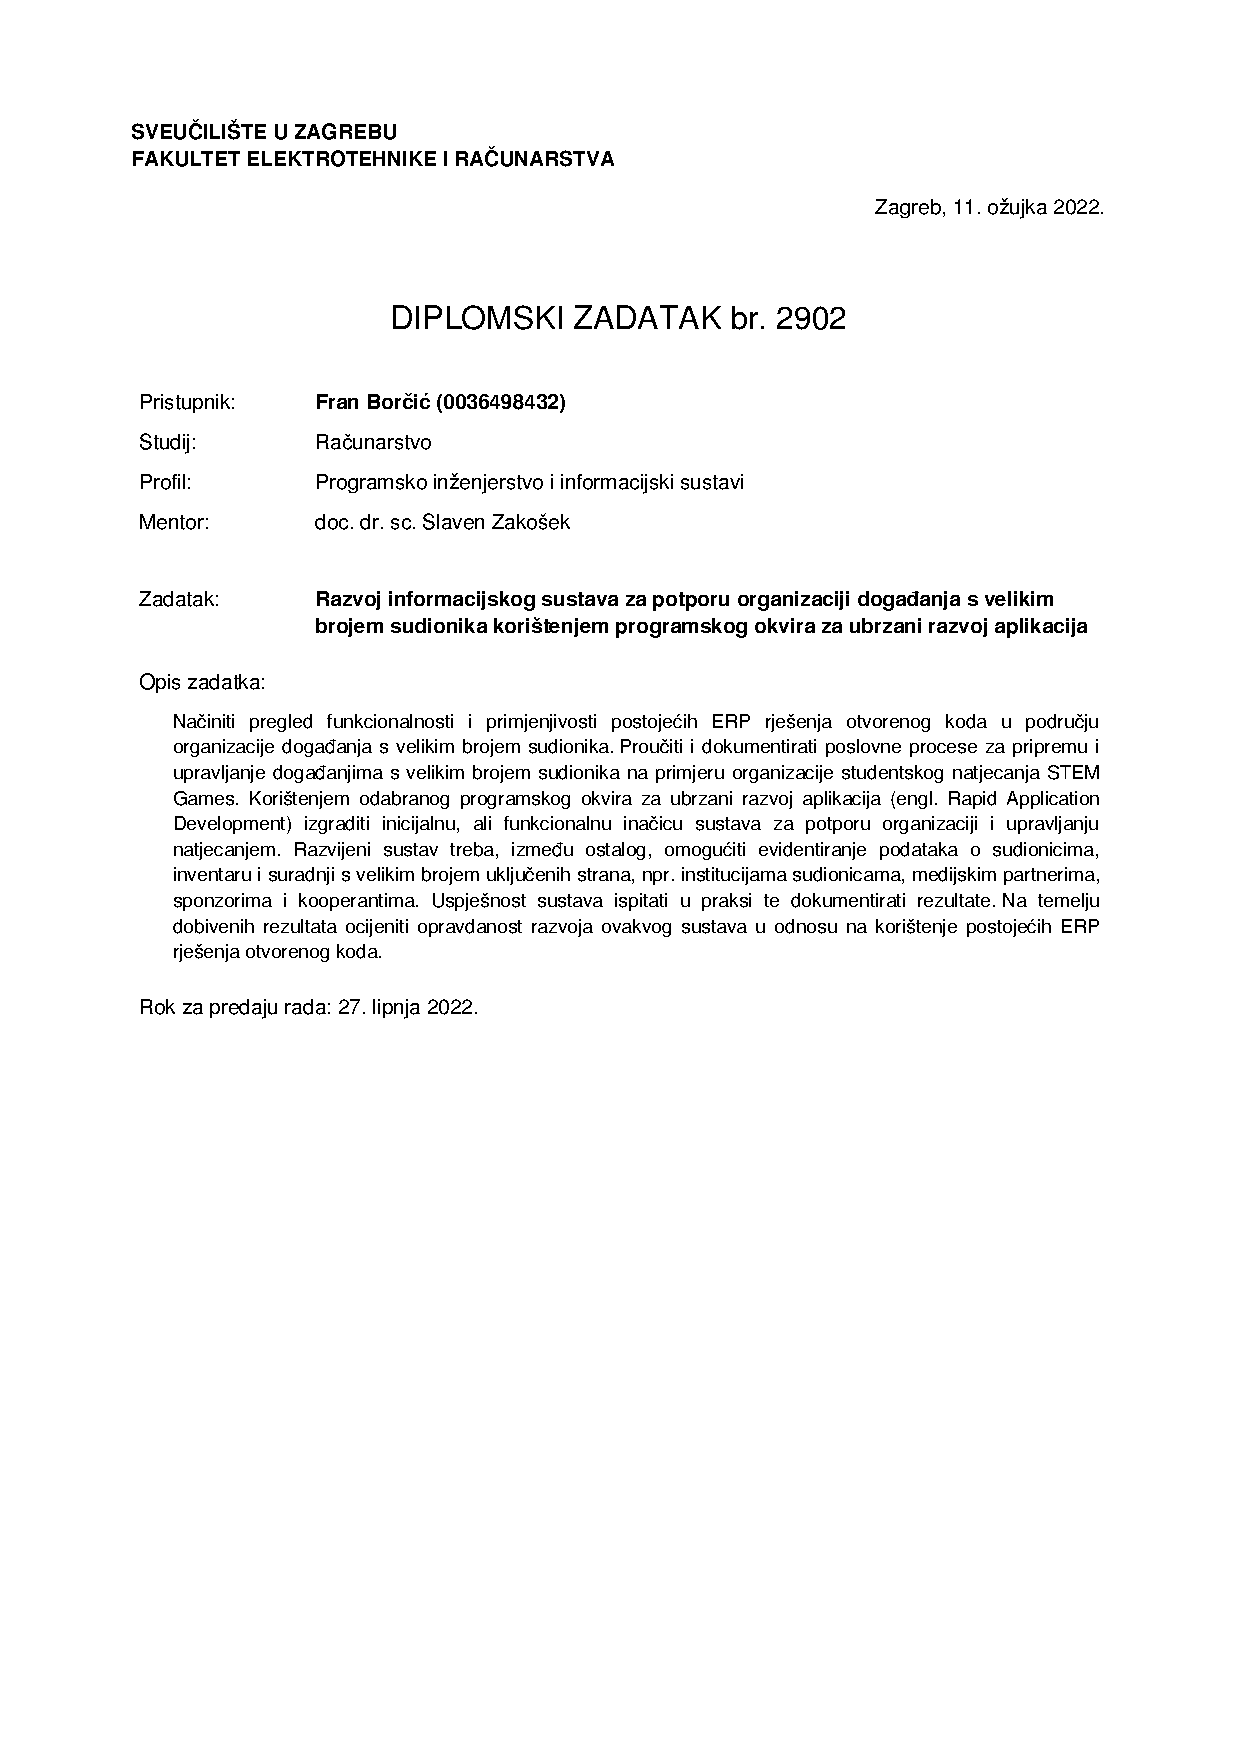
\includepdf{zadatak.pdf}

% \zahvala{}

\tableofcontents

\chapter{Uvod}

Cilj ovog rada je ocijeniti mogućnost i isplativost implementacije
infromacijskog sustava u rad studentskih organizacija koje se bave organizacijom
studentskih natjecanja s velikim brojem sudionika. Problemu će se pristupiti s
dva različita aspekta -- analizom prikladnosti postojećih rješenja i razvojem
osnovnog, ali primjenjivog prilagođenog rješenja koristeći programski okvir za
ubrzani razvoj aplikacija \engl{RAD}, a vodeći se konkretnim primjerom
\emph{Udruge za studentska natjecanja STEM Games}.

Tijekom posljednja nekoliko desetljeća svjedočimo sve većoj prisutnosti
informacijskih sustava u poslovanju komercijalnih organizacija, većinom u vidu
radnih okvira poznatih kao \emph{ERP} sustavi. Pojam \emph{ERP rješenje}
\engl{enterprise resource planning} obuhvaća veliki broj informacijskih sustava
različitih vrsta i primjena, no prema definicijama navedenima u
(\cite{evolutionerp})
taj se pojam odnosi na sustave koje karakterizira modularnost te centralizirana
pohrana svih podataka vezanih uz poslovanje jedne organizacije.

Većina takvih sustava danas je realizirana kao skup gotovih modula oblikovanih
prema generičkim potrebama većeg broja komercijalnih organizacija
(\cite{bradford2014modern}). S obzirom na broj poslovnih procesa prisutnih u
svakoj takvoj organizaciji, takva arhitektura omogućuje ubrzanu implementaciju
većeg dijela informacijskog sustava i ponovnu uporabu novorazvijenih modula u
organizacijama sličnog područja rada.

Logična je posljedica spomenute arhitekture da je uvođenje ERP sustava u
poslovanje to jeftinije i jednostavnije što je više poslovnih procesa organizacije
u koju se uvodi prisutno i u drugim organizacijama. Organizacije koje se bave
rijetkim i specifičnim zadacima ograničene su u broju dostupnih rješenja kojima
mogu digitalizirati svoje poslovanje pa je slijedom toga i isplativost njihove
informatizacije znatno manja.

Slučaj koji će u ovom radu biti proučen osim zbog svojih poslovnih procesa
specifičan je i prema svojim ciljevima -- organizacija studentskih natjecanja na
području RH tradicionalno je neprofitnog karaktera, a iza takvih događaja stoje
studentske udruge ili udruge građana čiji su članovi volonteri. Iz tog razloga,
potencijalni benefiti uvođenja informacijskog sustava u tom području očitovali
bi se prije svega u jednostavnosti obavljanja volonterskog rada, a u znatno
manjoj mjeri kroz financijske pokazatelje. Također, takve organizacije uglavnom
ne mogu u svojim budžetima opravdati profesionalnu izradu informacijskog
sustava, ali su im dostupni ljudski resursi u obliku studenata volontera.

Eventualni informacijski sustavi koji bi bili prikladni za takve organizacije,
bili bi osmišljeni tako da se studenti volonteri uz minimalnu edukaciju mogu
brinuti o uvođenju i održavanju takvih sustava. S obzirom na sličnosti u formatu
različitih studentskih natjecanja na području RH, kroz ovaj rad nastojat će se
pronaći rješenje koje bi olakšalo svih takvih događanja, a čija primjena bi
zahtjevala što manje tehničkog znanja.

Takvo što moglo bi se postići primjenom ERP rješenja otvorenog koda i prethodnom
pripremom njihove konfiguracije za konkretni zadatak organizacije. ERP rješenja
otvorenog koda za neprofitne organizacije postoje te će biti razmotrena u
nastavku rada, no s obzirom na činjenicu da se u ovom slučaju radi o vrlo
specifičnom tipu neprofitne organizacije takva rješenja ne mogu pokriti sve
njene potrebe.

Bolje prilagođeno rješenje, ali tehnički zahtjevnije za održavanje, moglo bi se
ostvariti korištenjem programskih okvira za ubrzani razvoj aplikacija
\engl{RAD}. Takvi programski okviri automatiziraju izradu čestih elemenata
korisničkog sučelja prema vezanom podatkovnom modelu te time omogućuju brzu
izradu programske potpore čiji je glavni zadatak pohrana podataka. Fokus ovog
rada upravo je razvoj ovakvog rješenja, ocjena njegove primjenjivosti te
potencijal za iskorištenjem u većem broju organizacija.

U poglavlju koje slijedi bit će opisane organizacijske strukture \emph{Udruge za
studentska natjecanja STEM Games} te njihovi zadaci prema podacima iz godišnjih
izvještaja različitih organizacijskih timova koji su sudjelovali na prethodnim
projektima te udruge. Ti će zadaci, odnosno poslovni procesi koje oni uključuju,
kasnije poslužiti za izolaciju zahtjeva na informacijski sustav koji bi pružao
podršku organizaciji studentskih natjecanja. Zatim će biti razmotrena dostupna
ERP rješenja otvorenog koda te broj zahtjeva koji bi se njihovom primjenom
zadovoljio, nakon ćega će biti opisano rješenje ostvareno koristeći RAD
programski okvir. Naposlijetku, razvijeno rješenje bit će empirički ocijenjeno
prema iskustvima unutar spomenutog STEM Games organizacijskog tima te će se
sažeti zaključci o primjenjivosti informacijskih sustava u organizacijama tog
tipa.

\chapter{Primjer strukture organizacije}

U ovom poglavlju, na primjeru udruge \emph{Udruge za studentska natjecanja STEM
Games} čiji je glavni projekt organizacija godišnjeg natjecanja za studente STEM
fakulteta pod imenom STEM Games, bit će opisane temeljne procedure potrebne za
organizaciju takvog događaja. Spomenuta organizacija, koju će se dalje u radu iz
praktičnih razloga zvati \emph{organizacija STEM Games}, poslužit će kao primjer
jer je autoru koji je u trenutku pisanja rada na njenom čelu dostupan veliki
broj podataka o dosadašnjim projektima udruge.

Zbog složenosti strukture organizacija ove vrste, praktičnije ju je opisati na
konkretnom primjeru organizacije koja se njome bavi. Dalje će se, međutim,
nastojati odvojiti koncepte proizašle iz opisa koji slijedi od konkretne STEM
Games organizacije, u skladu s nastojanjem da rezultati rada budu primjenjivi na
sve slične organizacije.

U svrhu lakšeg razumjevanja organizacije STEM Games, valja prvo ukratko opisati
događaj kojim se bavi.

\section{Natjecanje STEM Games}

Organizacija STEM Games nastala je i djeluje s ciljem da se studentima STEM
fakulteta omogući događanje na kojem se sudjelovanjem na natjecateljskim
aktivnostima mogu povezati s kolegama s drugih institucija te predstavnicima
industrije u njihovoj budućoj struci. Samo natjecanje osmišljeno je po modelu
već postojećih studentskih događanja u regiji, uz određene prilagodbe vezane
specifično uz STEM područje i suradnju s industrijom.

Organizacija jednom godišnje organizira natjecanje na kojem okuplja između
tisuću i dvije sudionika, odnosno petnaest do dvadeset visokoobrazovnih
institucija.  Studenti sudionci, prema kategorijama dostupnim u trenutku pisanja
ovog rada, natječu se u rješavanju problemskih zadataka STEM područja, sportskim
disciplinama ili računalnim igrama. Uz to, na prijedlog volontera organizira se
dodatni program u obliku neslužbenih natjecanja, predavanja, koncertnih
događanja i slično.

Središnji element ovog konkretnog natjecanja je tzv. \emph{natjecanje u znanju}
u kojem se timovi sudionika natječu u primjeni znanja stečenog na svojim
fakultetima. Radi se o četiri odvojena natjecanja u kojima se natječu timovi
studenata prirodoslovnog, tehnološkog, inžinjerskog ili matematičkog usmjerenja,
rješavajući probleme koji se u suradnji s predstavnicima industrije modeliraju
prema problemima s kojima će se sresti na budućem radnom mjestu.  \footnote{Taj
    element omogućuje financiranje organizacije kroz sponzorsku suradnju; u
    smislu ovog rada, bitno je uzeti u obzir da je ta mogućnost specifična za
    natjecanje u STEM području i da veći broj ostalih studentskih natjecanja ne
uključuje takav program.}

Glavne zadaće organizacije STEM Games uključuju omogućavanje provedbe svih
natjecateljskih elemenata, logističko i financijsko planiranje, prikupljanje
sredstava, pronalazak volontera, komunikaciju s institucijama sudionicama i
promotivne aktivnosti.

\section{Hijerarhijska struktura organizacije}

Zbog velikog opsega događanja, u organizaciji dosadašnjih izdanja svake je
godine dosad sudjelovalo oko 150 volontera. Kako bi se organizacijski tim te
veličine uspješno koordinirao, organizacija je ustrojena hijerarhijski te dijeli
volontere u različite timove ovisno o zadatku kojim se bave.

Na slici \ref{fig:hier} prikazana je podjela organizacije po timovima čiji će
zadaci biti opisani u nastavku. Cjelokupnu organizaciju koordiniraju dva
\emph{voditelja organizacije} uz pomoć voditelja pojedinih organizacijskih
timova, u kojima je također prisutan interni ustroj. Detalji ustroja timova za
svrhe ovog rada nisu relevantni, no gruba podjela organizacije prikazana je kako
bi se u nastavku organizacijski zadaci mogli smisleno podijeliti po timovima
koji ih izvršavaju.

U potpoglavljima koja slijede po timovima će biti opisani oni njihovi zadaci u
čijoj provedbi potencijalni informacijski sustav može biti koristan.

\begin{figure}[H]
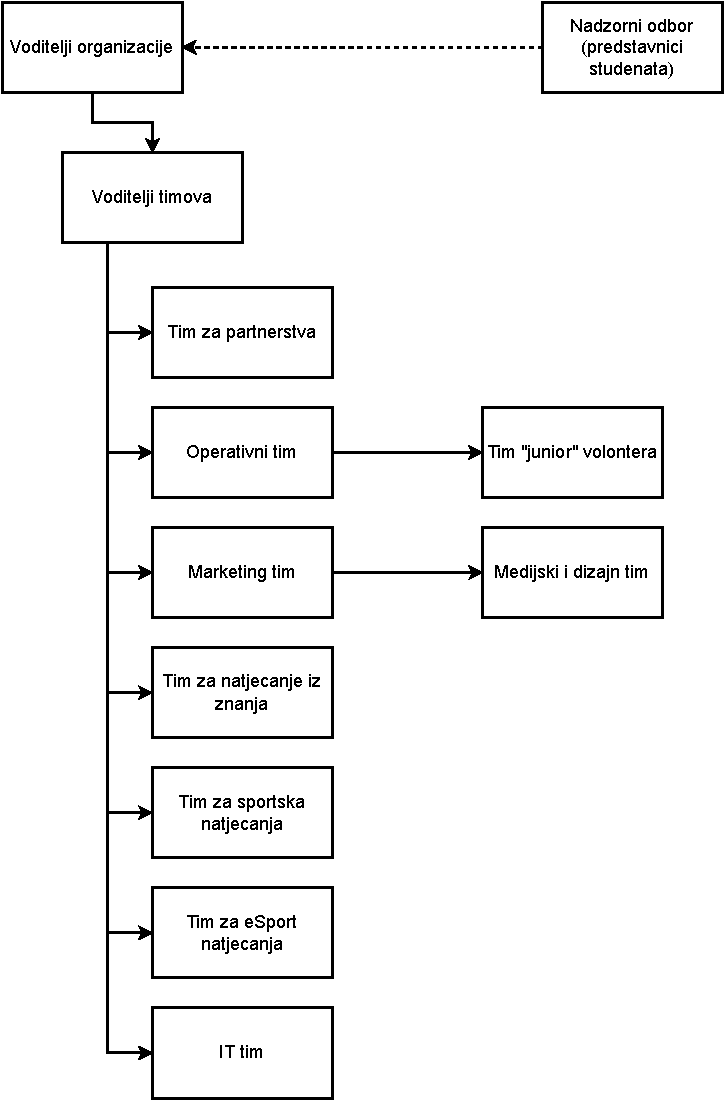
\includegraphics{slike/hijerarhija.pdf}
\caption{Prikaz organizacijskog ustroja}
\label{fig:hier}
\end{figure}

\section{Zadaci voditelja organizacije}
Voditelji organizacije, za koje su predviđene dvije pozicije u organizacijskoj
strukturi, započinju organizaciju projekta početkom akademske godine. Zaduženi
su, najprije, za okupljanje predstavnika studenata institucija koje će
sudjelovati.

Predstavnici onih institucija koje su dosad sudjelovale na natjecanju čine tzv.
\emph{nadzorni odbor} koji potvrđuje voditelje organizacije za tu godinu.
Voditelji organizacije potom digitalnim putem objavljuju natječaj za volontere u
organizaciji, od kojih se biraju drugi članovi organizacije uz potvrdu nadzornog
odbora.

Nakon ustroja organizacijskog tima, voditelji organizacije zaduženi su za
vremensko i resursno planiranje organizacije. Moraju voditi računa o
potencijalnim izvorima financiranja i rashodima potrebnima za organizaciju,
konzultirati nadzorni odbor o željama sudionika te ih uzeti u obzir prilikom
planiranja zadataka za organizacijske timove. Također, brinu se o suradnji s
kooperantom koji omogućuje prostor u kojem će se odvijati natjecanje te
posreduju u komunikaciji između ugostitelja i predstavnika institucija
sudionica.

Osim toga, voditelji organizacije brinu se o neprofitnoj organizaciji koja stoji
iza organizacijskog tima natjecanja. Brinu se o ispravnom bilježenju prihoda i
rashoda u suradnji s računovodstvenim servisom, ugovorima sa sponzorima i
kooperantima, održavanju skupština udruge i općenitim administrativnim poslovima
koji su za nju vezani.

\section{Zadaci studentskih predstavnika}

Studentski predstavnici posreduju u komunikaciji između organizacijskog tima i
studenata visokoobrazovnih institucija koje sudjeluju na natjecanju. Prema
prethodnom sudjelovanju, neki od predstavnika studenata imaju pravo glasati o
pitanjima vezanim uz tijek organizacije. To čine digitalnim putem ili na
sastancima nadzornog odbora koje sazivaju voditelji organizacije.

Predstavnici također biraju studente koje će njihova institucija povesti na
natjecanje nakon što se studenti prijave preko jedinstvene stranice
organizacije. Zaduženi su i za organizaciju prijevoza sudionika na događaj te
eventualnog sufinanciranja njihovog sudjelovanja fakultetskim ili sponzorskim
subvencijama.

\section{Zadaci operativnog tima}

Operativni tim kao organizacijski tim u užem smislu ima veliki broj zadaća, te
je možda više od bilo kojeg drugog tima podložan informatizaciji. Glavne zadaće
operativnog tima su briga o nabavi, upravljanje inventarom, organizacija
lokalnog prijevoza, upravljanje timom "junior" volontera\footnote{volontera koji
    ne sudjeluju u organizaciji, ali pomažu fizički u provedbi samog događaja},
    organizacija dodatnog programa, akreditacija sudionika te briga o rasporedu
    događanja.

Detaljni zahtjevi na informacijski sustav od strane ovog tima, kao i drugih
timova, bit će opisani u nastavku, no ovdje vrijedi nešto detaljnije opisati
pojedinosti nabrojanih zadaća.

\subsection{Nabava i upravljanje inventarom}
Operativni tim vodi evidenciju o svim kooperantima s kojima je ostvarena
komunikacija tijekom tekućeg i prijašnjih projekata te prema tome ostvaruje
suradnje nužne za provedbu događaja. Ostali timovi iskazuju svoje potrebe za
nabavom materijala operativnom timu te članovi operativnog tima komuniciraju s
potencijalnim dobavljačima i dogovaraju nabavu. Nabavu u skladu s definiranim
budžetom odobravaju voditelji organizacije.

Veliki dio nabave potrebne za projekt odnosi se na tiskane materijale, koji se
tijekom događaja koriste za promociju sponzora i informiranje sudionika.
Prilikom nabave tiskanih materijala operativni tim mora, osim s dobavljačima,
komunicirati s \emph{timom za partnerstva} koji se brine o odobrenju materijala u
kojima se spominju sponzori događaja te \emph{medijskim i dizajn timom} koji
priprema grafičke pripreme.

Tijekom događaja, tim upravlja svim inventarom koji se koristi za provedbu
natjecanja. Brine o vlasništvu inventarskih stavki (one mogu biti posuđene, u
vlasništvu udruge, volontera ili ugostiteljima), zaduženjima i ovlastima među
volonterima te lokacijama na kojima se pojedini predmeti u svakom trenutku
nalaze. Također brinu o prijevozu tih predmeta na lokaciju i njihovom povratku
vlasnicima.

\subsection{Lokalni prijevoz i prijevoz organizacije}

Jedan od zadataka operativnog tima također je osigurati prijevoz organizatora na
mjesto događaja. Pritom mora voditi računa o lokaciji polaska različitih članova
organizacije i rasporedu njihovog dolaska po danima.

Na lokaciji natjecanja mora brinuti o zaduženjima službenih vozila u najmu i
prioritetima za njihovo korištenje. Također, mora koordinirati autobusni
prijevoz sudionika u različitim komponentama natjecanja do sportskih dvorana ili
dvorana u kojima se odvija natjecanje u znanju.

\subsection{Upravljanje sudionicima}

Operativni tim zadužen je također za provedbu prijava sudionika preko web
sučelja na stranicama organizacije, komunicirajući pritom s predstavnicima
studenata o njihovim procedurama selekcije i kategorijama za koje žele otvoriti
prijave. Nakon selekcija provedenih od strane matičnih institucija sudionika,
operativni tim brine o njihovim osobnim podacima, izdaje ulaznice za događaj,
brine o njihovom dolasku i odlasku te posreduje u komunikaciji s ugostiteljskom
tvrtkom.

\subsection{Dodatni program, raspored i "junior" volonteri}

\section{Zadaci tima za partnerstva}
\section{Zadaci tima za marketing i komunikacije te podtimova}
\section{Ostale potrebe}

\chapter{Zahtjevi na sustav}
\chapter{Dostupni \emph{ERP} sustavi otvorenog koda}
\chapter{Rješenje primjenom \emph{RAD} programskog okvira}

\chapter{Zaključak}
...
\bibliography{literatura}
\bibliographystyle{fer}

\begin{sazetak}
Sažetak na hrvatskom jeziku.

\kljucnerijeci{Ključne riječi, odvojene zarezima.}
\end{sazetak}

% TODO: Navedite naslov na engleskom jeziku.
\engtitle{Title}
\begin{abstract}
Abstract.

\keywords{Keywords.}
\end{abstract}

\end{document}
